\section{Results}\label{sec:results}
This section evaluates the benchmarked policies across RQ1--RQ4, progressing from decision-layer information and cost noise (Sec.~\ref{sec:rq1}) and strategic incentives (Sec.~\ref{sec:rq2}) to execution-layer channel and map resilience (Sec.~\ref{sec:rq3}) and multi-robot 3D Gazebo transfer (Sec.~\ref{sec:rq4}).

\subsection{Information, Geometry, Cost Noise, and Generalization (RQ1)}\label{sec:rq1}
The single-bay baseline (\texttt{S1}, with 7 bay positions $\times$ 60 seeds = 420 episodes per policy) first tests whether inter-robot communication is necessary. Without communication, the \texttt{reactive} baseline succeeded in $93.8\%$ [91.1--95.7\%] of encounters, deadlocking in the remaining 26 episodes when random patience timers failed to break symmetry before the $180$\,s time limit. Even when successful, \texttt{reactive} was slow and inefficient; it averaged $97.1\pm4.5$\,s of total delay against $26.8\pm0.6$\,s for the hindsight reference, a $3.6\times$ penalty. Because the 26 deadlocked episodes are excluded, this is a lower bound; charging both robots the full $180$\,s in every deadlocked episode bounds the mean at $113$\,s ($4.2\times$). Because the robots could not coordinate their intent, both backed up simultaneously in $39\%$ of episodes, driving an average of $5.7$\,m in reverse versus $0.64$\,m for the reference. By contrast, all four negotiating policies in \texttt{S1} (\texttt{fixed\_priority}, \texttt{rules\_default}, \texttt{rules\_proximity}, and \cb) completed $100\%$ of episodes (420/420) with zero collisions. Although \texttt{fixed\_priority} could in principle operate without radio if robot IDs were sensed visually, here it uses the broadcast protocol; thus, its gain over \texttt{reactive} reflects the combined benefit of a shared tie-breaking rule and explicit message passing. A stronger zero-communication baseline, randomized exponential backoff (\texttt{backoff}, patience drawn from $U[0, 6\cdot2^{k}]$\,s after $k$ earlier yields; study \texttt{S11b}), raises completion to $96.7\%$ but not efficiency ($92.3\pm6.3$\,s excess delay vs.\ $6.5\pm0.6$\,s for \texttt{fixed\_priority}). One-at-a-time sweeps of every rulebook threshold on the \texttt{S1}, \texttt{S2}, and \texttt{S4} grids (\texttt{S11a}) left excess delay unchanged except for the urgency threshold, which at $2.5$ raises \texttt{S2} weighted excess from $3.5$ to $15.7$\,s (\texttt{rules\_default}).

While any shared tie-breaking rule eliminates symmetric deadlocks, encounter efficiency depends strongly on how policies exploit corridor geometry. Figure~\ref{fig:rq1_geom} shows how excess delay $\Delta_\pi$ varies with pull-in bay position $x\in\{1,\dots,7\}$\,m for symmetric robots. Under \texttt{fixed\_priority} and \texttt{rules\_default} (which coincide when robots have equal urgency and load, because robot $A$ always enters at $t=0$ ahead of delayed robot $B$), excess delay averages $6.4\pm 0.6$\,s overall, spiking to $14.6$--$14.8$\,s when the bay sits near $A$'s entrance ($x=2$--$3$\,m), where $B$ is forced to reverse all the way back to \texttt{room\_hi} even when $A$ has just passed a nearby bay. Promoting geometric proximity ahead of corridor seniority (\texttt{rules\_proximity}) halves overall excess delay to $3.1\pm 0.5$\,s. Residual peaks remain at $x=3$\,m ($14.8$\,s) and $x=4$\,m ($7.1$\,s), where \texttt{rules\_proximity} makes exactly the same choices as \texttt{fixed\_priority}: $A$ has slightly passed the bay at conflict detection, yet reversing $A$ into it remains cheaper than reversing $B$ out of the aisle. This advantage is layout-specific: in the two-bay corridor (\texttt{S4}, 360 encounters), \texttt{rules\_proximity} incurs $5.6\pm 0.5$\,s of excess delay and picks the hindsight yielder in only $14\%$ of encounters, worse than both \texttt{fixed\_priority} ($1.1\pm 0.3$\,s) and \texttt{rules\_default} ($1.2\pm 0.3$\,s), because the nearest refuge is often not the cheaper one when a second bay is available.

\begin{figure}[!t]\centering
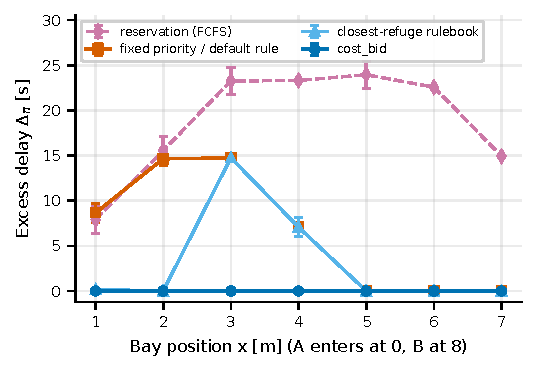
\includegraphics[width=\columnwidth]{Images/fig5_bay_geometry.pdf}
\caption{Mean excess delay $\Delta_\pi$~\eqref{eq:excess} versus pull-in bay coordinate $x$ in the single-bay corridor across negotiating policies (\texttt{S1}) and first-come corridor mutex locking (\texttt{reservation}). Error bars show 95\% CIs.}
\label{fig:rq1_geom}
\end{figure}

By comparison, coarse corridor-level locking ignores intermediate pull-in bays altogether. First-come corridor reservation (\texttt{reservation}, evaluated over 210 encounters across $x\in\{1,\dots,7\}$\,m in Fig.~\ref{fig:rq1_geom}) completed $100\%$ of episodes without collision, but incurred $18.8\pm 0.9$\,s of excess delay. This delay is nearly triple that of \texttt{fixed\_priority} ($6.5\pm 0.9$\,s on the same draws), and \texttt{reservation} never outperformed the best forced yielder ($0/210$ encounters). Because Robot~$B$ starts directly on Robot~$A$'s exit path, waiting outside the corridor forces $B$ to turn and park off-lane inside \texttt{room\_hi} (adding $\sim 17$\,s of maneuver overhead) while waiting for $A$ to traverse the entire aisle rather than using an intermediate bay. Facility layouts where staging areas already sit clear of the exit lane would penalize reservation less severely. At the other extreme, noise-free \cb\ selected the exact same yielder as the hindsight reference in $100\%$ of single-bay (\texttt{S1}, 420 encounters) and two-bay (\texttt{S4}, 360 encounters) episodes ($\Delta_\pi = 0.0$\,s). Because \cb\ uses the true speed limits and refuge coordinates of the deterministic simulator, this exact match primarily validates the cost model. Omitting acceleration and turning transients produces a mean absolute prediction error of $1.9$\,s per robot (up to $4.0$\,s across 780 episodes), yet in symmetric corridors that error is never large enough to flip which robot should yield.

\begin{figure}[!t]\centering
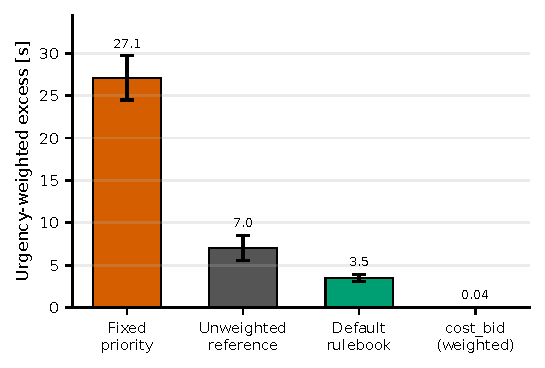
\includegraphics[width=\columnwidth]{Images/fig6_asymmetry.pdf}
\caption{Urgency-weighted excess delay across heterogeneous robot urgency, payload, and speed regimes (\texttt{S2}, $N=5{,}040$). Error bars show 95\% CIs.}
\label{fig:rq1_asym}
\end{figure}

Moving from identical robots to mixed fleets highlights the trade-off between simple priority rules and estimating actual maneuver delays. In study \texttt{S2} (5,040 episodes, Fig.~\ref{fig:rq1_asym}), where robots differ in urgency ($u_B\in\{1,3\}$), payload status, and top speed ($v_B\in\{0.26,0.13\}$\,m/s), static ID priority (\texttt{fixed\_priority}) performs poorly. It incurs $27.1\pm 2.6$\,s of urgency-weighted excess delay because Robot~$B$ is forced into long reverse maneuvers even when carrying an urgent load or moving at half speed. Adding simple urgency and payload rules (\texttt{rules\_default}) reduces this weighted excess delay nearly eightfold to $3.5\pm 0.4$\,s. Crucially, the hindsight reference that minimizes \emph{unweighted} total delay (\texttt{oracle}) still incurs $7.0\pm 1.5$\,s of urgency-weighted excess delay. Thus, optimizing the wrong fleet objective wastes twice as much weighted time as replacing a kinematic planner with a heuristic rulebook. By contrast, urgency-weighted \cb\ reduces weighted excess delay to just $0.04\pm 0.02$\,s and picks the same yielder as the weighted reference (\texttt{oracle\_w}) in $98\%$ of encounters (704/720). The 16 remaining encounters are all close near-ties where unmodeled acceleration and turning transients slightly shift the outcome, having a median predicted bid difference of only $0.6$\,s (maximum $2.2$\,s) compared with $12.4$\,s across the 704 agreed encounters.

In real-world deployments, however, robots cannot predict their maneuver delays exactly due to floor friction, battery sag, and localization jitter. To test how sensitive \cb\ is to estimation errors, study \texttt{S7} (single-bay corridor, Fig.~\ref{fig:rq1_noise}) multiplies each robot's predicted bid by log-normal noise $e^{\sigma\epsilon}$. As the noise level $\sigma$ increases, the excess delay of \cb\ rises from $0.0$\,s ($\sigma=0$) to $0.15\pm 0.15$\,s ($\sigma=0.1$), $1.5\pm 0.6$\,s ($\sigma=0.25$), $3.3\pm 0.8$\,s ($\sigma=0.5$), and $4.5\pm 0.9$\,s ($\sigma=1.0$). Once bid noise reaches $\sigma=0.5$ (where bids typically vary by a factor of $e^{0.5}\approx 1.65\times$), noisy \cb\ offers no statistical advantage over the simple closest-refuge rulebook (\texttt{rules\_proximity}, $3.2\pm 0.8$\,s on the same draws), and remains clearly better only when $\sigma\le 0.25$; at $\sigma=1.0$ the rulebook is ahead by a paired $1.3\pm 1.2$\,s. Because \texttt{rules\_proximity} itself trails fixed priority in the two-bay layout, this crossover should not be generalized beyond single-bay corridors. Note that study \texttt{S7} adds random noise to the final bid value, whereas systematic model errors (such as a miscalibrated reverse speed $v_{\mathrm{rev}}$) remain an open direction for future testing.

\begin{figure}[!t]\centering
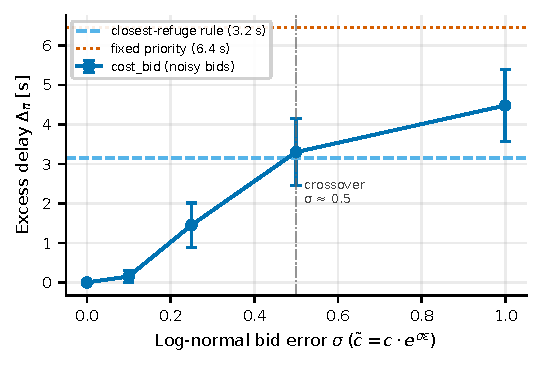
\includegraphics[width=\columnwidth]{Images/fig7_bid_noise.pdf}
\caption{Sensitivity of \cb\ excess delay $\Delta_\pi$ to multiplicative log-normal bid estimation error $\sigma$ (\texttt{S7}, $N=3{,}150$), reaching parity with noise-free \texttt{rules\_proximity} at $\sigma\approx 0.5$. Error bars show 95\% CIs.}
\label{fig:rq1_noise}
\end{figure}

Instead of using a formula to estimate maneuver delays, a policy can learn which robot should yield directly from past encounters. Figure~\ref{fig:rq1_bandit} shows that on the two-bay corridor layout where it was trained, the tabular full-information outcome classifier (\texttt{learned}) matches the performance of \texttt{rules\_default} on held-out test episodes ($+2.6$\,s vs.\ $+2.5$\,s weighted excess delay; a table trained on only $200$ encounters already reaches $+2.8$\,s) without relying on an explicit motion model. However, when tested on an unseen single-bay corridor with randomized bay positions, its excess delay jumps to $+13.1$\,s. This performance is worse than both \texttt{fixed\_priority} ($+12.3$\,s) and \texttt{rules\_default} ($+6.3$\,s), with $15\%$ of encounters falling into state bins never seen during training. Because the classifier only looks at coarse distance bins to the nearest refuge behind each robot and ignores where the oncoming robot can stop relative to each bay, the lookup table memorizes layout-specific patterns rather than general corridor physics.

\begin{figure}[!t]\centering
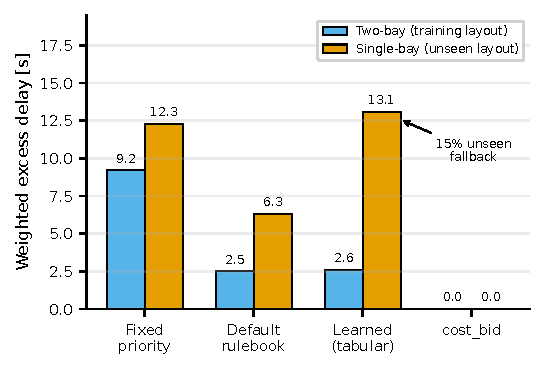
\includegraphics[width=\columnwidth]{Images/fig8_bandit_generalization.pdf}
\caption{Tabular outcome classifier (\texttt{learned}) weighted excess delay on its training two-bay layout versus an unseen single-bay layout ($150$ evaluation episodes per layout).}
\label{fig:rq1_bandit}
\end{figure}



\subsection{Strategic Incentives and Repeated-Encounter Fairness (RQ2)}\label{sec:rq2}
The strong performance of \cb\ in Section~\ref{sec:rq1} assumes that every robot reports its delay cost honestly. In a multi-vendor facility, however, a self-interested robot can exaggerate its predicted delay to avoid yielding. In study \texttt{S6} (1,080 episodes), where the lower bid yields without any payment, if Robot~$B$ multiplies its reported bid by $k\ge 2\times$, it forces Robot~$A$ to yield in $100\%$ of encounters. As a result, $B$'s own mean delay drops from $9.1\pm 1.4$\,s to $8.1\pm 1.2$\,s, while the combined fleet delay increases by $+4.9$\,s ($+20\%$). Similarly, in the unpriced baseline of study \texttt{S9} (dashed orange curve in Fig.~\ref{fig:rq2_misreport}), Robot~$A$ gains up to $+4.74\pm 0.99$\,s of individual utility by inflating its bid by $k=4\times$. Simply making the proceeding robot pay the yielding robot's reported bid does not encourage honesty either. Instead, this naive side-payment reverses the incentive to lie (dotted purple curve in Fig.~\ref{fig:rq2_misreport}), allowing Robot~$A$ to gain $+7.54\pm 1.76$\,s by \emph{under-reporting} its cost at $k=0.25\times$ to manipulate the payment terms, while Robot~$B$ gains $+0.68$\,s at $k=0.75\times$.

\begin{figure}[!t]\centering
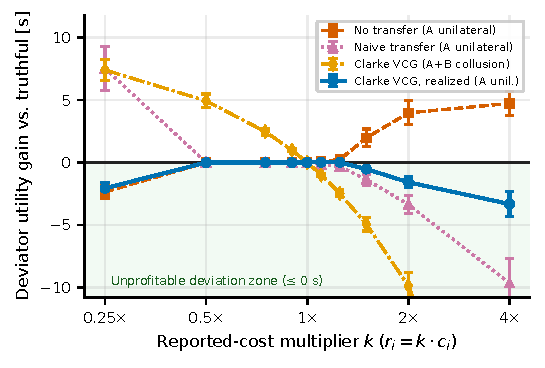
\includegraphics[width=\columnwidth]{Images/fig9_strategic_misreport.pdf}
\caption{Deviator single-encounter utility gain (seconds of urgency-weighted delay plus transfer) relative to truthful reporting ($k=1\times$) across $N=10{,}080$ episodes in \texttt{S9}; values $\le 0$\,s (shaded green) indicate unprofitable deviations. Error bars show 95\% CIs.}
\label{fig:rq2_misreport}
\end{figure}

To make honest reporting the best choice for each individual robot, study \texttt{S9} evaluates the Clarke-pivot mechanism (Eq.~\eqref{eq:clarke}) across 6 bay and urgency settings, 27 unilateral and joint misreport conditions (deviator $\in\{A, B, AB\}\times$ nine non-truthful scales $k\in\{0.25, 0.5, 0.75, 0.9, 1.1, 1.25, 1.5, 2, 4\}$) plus the truthful baseline ($k=1$), and 60 seeds (10,080 episodes total, all completing without collision). Under the planner's predicted costs, \emph{no} single-robot misreport ($0/108$ deviator conditions across Robots~$A$ and~$B$) improves the lying robot's utility ($0.00$\,s maximum gain), confirming that truthful bidding is an exact dominant strategy. When utility is measured using the \emph{actual} simulated travel times (which differ slightly from the planner's predictions due to acceleration and turning transients), lying unilaterally costs Robot~$A$ up to $-3.3\pm 1.0$\,s of utility at extreme scaling factors (solid blue curve in Fig.~\ref{fig:rq2_misreport}) and Robot~$B$ up to $-4.9\pm 1.2$\,s (at $k=0.25\times$). Across the entire test grid, the largest realized gain from misreporting is just $+0.02\pm 0.02$\,s (at $k=1.1\times$), which is statistically indistinguishable from zero. Because both robots' types are computed from shared kinematic snapshots, this result is an implementation check of the mechanism rather than evidence of robustness to private information. With private urgency and independent per-outcome misreports (\texttt{S9b}, 10,080 deviating episodes), no deviation improved the deviator's predicted utility; realized gains above $0.01$\,s occurred in 89 episodes ($0.9\%$), all caused by execution departing from the predicted plan, and the mean realized gain was negative in every arm.


\begin{figure}[!t]\centering
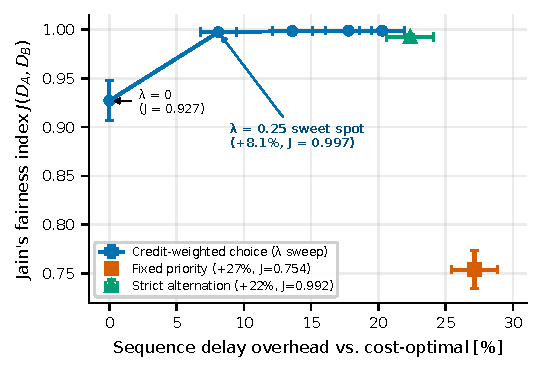
\includegraphics[width=\columnwidth]{Images/fig10_fairness_pareto.pdf}
\caption{Repeated-encounter Pareto frontier (\texttt{S10}, 50 sequences of 20 encounters) trading sequence delay overhead against cumulative Jain fairness $J(D_A^{\mathrm{cum}}, D_B^{\mathrm{cum}})$ as credit weight $\lambda$~\eqref{eq:karma} varies from $0$ to $2.0$. Error bars show 95\% CIs.}
\label{fig:rq2_fairness}
\end{figure}

At the same time, study \texttt{S9} highlights three practical limitations that fleet engineers must consider before deploying a Clarke-pivot (VCG) mechanism.
\begin{enumerate}
\item \emph{Chronic budget surplus.} In line with the Green--Laffont impossibility theorem~\cite{green1977characterization}, payments cannot simply be transferred from one encountering robot to the other and must instead be paid into an external fleet bank. This bank collects an average surplus of $9.3\pm 1.6$\,s of delay credit per encounter when $u_B=1$ ($44\%$ of the planner-predicted total delay cost, or $37\%$ of the realized urgency-weighted delay) and $10.5\pm 1.5$\,s when $u_B=3$ ($29\%$ predicted, $24\%$ realized), meaning the facility must periodically redistribute accumulated credits outside the real-time negotiation loop.
\item \emph{Vulnerability to joint collusion.} If Robot~$A$ and Robot~$B$ both scale their reported costs down by the same factor $k<1$, the chosen yielder $o^\ast$ stays the same while both robots' payments shrink by a factor of $k$. Under joint $0.5\times$ bid shading, their combined utility improves by $+4.94\pm 0.55$\,s (and by $+7.42$\,s at $0.25\times$, shown by the dash-dotted gold curve in Fig.~\ref{fig:rq2_misreport}).
\item \emph{Mandatory participation and non-bid cheating.} Compared with a static \texttt{fixed\_priority} policy where Robot~$A$ always has the right-of-way and pays nothing, Robot~$A$ is worse off under the Clarke mechanism in $100\%$ of encounters (losing an average of $9.3$\,s per encounter at $u_B=1$ and $10.5$\,s at $u_B=3$). Thus, high-priority robots will only participate if required by the facility operator. Furthermore, VCG only guarantees honesty for the reported cost numbers $b_i(o)$ and assumes robots follow the protocol honestly in other respects. A robot could still cheat outside the bidding math by omitting a known pull-in bay from its \texttt{BID} message to shrink the feasible refuge set $\mathcal{F}$, or by spoofing a lower robot ID to win \texttt{commit} tie-breakers.
\end{enumerate}

While multi-vendor fleets need payment mechanisms to ensure truthful bidding, single-owner cooperative fleets already share a common goal, yet can still suffer from unfair delays across repeated encounters if tie-breaking rules always favor the same robot. Across 50 sequences of 20 random single-bay encounters (study \texttt{S10}, Fig.~\ref{fig:rq2_fairness}), \texttt{fixed\_priority} forces Robot~$B$ to yield every time. This one-sided rule drops cumulative Jain fairness to $J=0.754$ while increasing total fleet delay by $+27.1\%$ compared with cost-optimal selection. Notably, pure cost-optimal selection ($\lambda=0$) already achieves high fairness ($J=0.927$) because random bay locations and start delays naturally vary which robot is closer to a refuge. Forcing the robots to strictly take turns yielding (\texttt{alternate}) raises fairness to $J=0.992$, but adds $+22.3\%$ of extra delay because it ignores corridor geometry. Choosing the fairness weight in Eq.~\eqref{eq:karma} on these 50 sequences (smallest-overhead $\lambda$ with $J\ge0.99$, giving $\lambda=0.1$) and evaluating it closed-loop on 100 fresh sequences (\texttt{S10b}) yields $J=0.992$ at $+3.8\pm0.6\%$ extra delay; with log-normal error on the delay estimates the overhead grows to $+7.1\%$ ($\sigma=0.25$) and $+11.5\%$ ($\sigma=0.5$) at unchanged $J\approx0.99$. The absolute-gap variant $\lambda\,|(D_A+d_A(o))-(D_B+d_B(o))|$ selects $\lambda=0.25$ and gives $J=0.994$ at $+3.0\%$. With a small $\lambda$, the rule follows the cost-optimal decision on clear-cut encounters and only flips close near-ties in favor of whichever robot has accumulated more past delay. This cumulative-delay ledger is kept strictly separate from the Clarke VCG payments in study \texttt{S9}, because carrying VCG credits over as a spending budget across multiple encounters would break the single-encounter truthfulness guarantee.


\subsection{Channel Impairment, Safeguard Ablation, and Map Uncertainty (RQ3)}\label{sec:rq3}
Having evaluated the decision policies under ideal communication, the next experiments test how the distributed execution protocol holds up when wireless links degrade. Across both moderate and heavy channel impairment in study \texttt{S3} (packet loss from $0\%$ to $90\%$ and latency from $0.05$\,s to $2.0$\,s over 3,600 episodes) and study \texttt{S8} (detection range $R_{\mathrm{det}}\in\{6,3,1.5\}$\,m, top speed $v_{\max}\in\{0.26,0.5\}$\,m/s, packet loss up to $90\%$, and latency up to $2.0$\,s over 4,320 episodes), every negotiating policy (\texttt{fixed\_priority}, \texttt{rules\_default}, \texttt{rules\_proximity}, and \cb) completed $\ge 99.3\%$ of encounters pooled over each study's grid (the hardest individual cells, at $90\%$ loss, still reached $\ge 90\%$) with \emph{zero collisions} (Fig.~\ref{fig:rq3_comms}). Mean delay stayed nearly flat (varying by only $1$--$2$\,s) up to $50\%$ packet loss because resending \texttt{BID} messages every $0.3$\,s reliably delivers both snapshots well before the robots physically meet. Delay rises gradually only above $70\%$ packet loss, where the $3.0$\,s negotiation timeout occasionally expires and triggers a reactive backoff fallback. Completion therefore overstates how often negotiation itself succeeds: at the most extreme loss levels of \texttt{S8b}/\texttt{S8c}, $62.8\%$ of episodes recorded no negotiated decision and were resolved by the reactive fallback. On fresh seeds with correlated loss (study \texttt{S8d}, 2,560 episodes; Gilbert--Elliott bursts of mean length 5--100 messages and total blackouts of 10--40\,s), no collision occurred and $\ge 99.4\%$ of encounters completed, but only $71.9\%$ of bursty-loss and $92.5\%$ of blackout episodes reached a negotiated decision.

\begin{figure}[!t]\centering
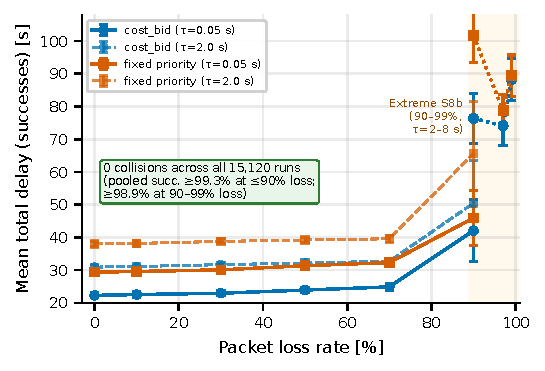
\includegraphics[width=\columnwidth]{Images/fig11_comms_resilience.pdf}
\caption{Mean total delay over successful episodes across packet loss $0$--$99\%$ and base latency $\tau\in[0.05, 8.0]$\,s (\texttt{S3} at $0.26$\,m/s and extreme \texttt{S8b} shaded right at $0.50$\,m/s); zero collisions occurred across all 15,120 communication-sweep and ablation episodes. Error bars show 95\% CIs.}
\label{fig:rq3_comms}
\end{figure}

Under extreme channel impairment in study \texttt{S8b} ($90\%$ to $99\%$ packet loss, $2$\,s to $8$\,s latency, and $v_{\max}=0.5$\,m/s across 1,440 episodes), an early version of the agent experienced 6 collisions when both robots yielded on mismatched snapshots and pulled back out into the corridor at the same time. After tightening the lane-clearance and bay-exit checks in the final protocol, all four negotiating policies recorded \emph{zero collisions} across all 1,440 episodes in \texttt{S8b}, achieving $98.9\%$ to $99.2\%$ completion. (Note that studies \texttt{S8b} and \texttt{S8c} used a higher top speed of $0.5$\,m/s in 2D to stress-test fast closing speeds, whereas the extreme-communication runs in Gazebo used the standard TurtleBot3 Waffle speed of $0.26$\,m/s.)

To test which protocol safeguard actually prevents collisions, study \texttt{S8c} (Table~\ref{tab:abl}, 5,760 episodes) turns \texttt{commit}, \texttt{state\_guard}, and \texttt{bay\_check} on and off in all $2^3$ combinations under the extreme packet-loss and latency settings of study \texttt{S8b}. Surprisingly, \emph{zero collisions occurred in every single test condition}, even when all three safeguards were turned off ($95\%$ upper bound of $1.06\%$ per 360-episode condition). Two factors explain why disabling the radio safeguards did not cause collisions. First, at a $5$\,Hz broadcast rate and $90\%$ to $99\%$ packet loss, the chance that a robot has no fresh ($<1$\,s) peer \texttt{STATE} message is $0.90^5=59\%$ to $0.99^5=95\%$, and any messages that do arrive are already $2$\,s to $8$\,s old. Physical collision avoidance under extreme loss therefore comes from local Lidar stopping margins and randomized $U[6,12]$\,s bay-exit wait timers rather than radio-based state guards. Second, \texttt{bay\_check} never triggered even once (all 8 conditions with \texttt{bay\_check} enabled produced the exact same episode outcomes as those with it disabled). Meanwhile, turning on \texttt{commit} added $3.1$\,s to $3.8$\,s of mean delay and actually \emph{increased} how often both robots started yielding at the same time (from $15.3\%$--$16.4\%$ to $21.9\%$--$23.6\%$ under \texttt{fixed\_priority}), because waiting for a dropped confirmation packet pushes robots past the $3.0$\,s negotiation timeout into reactive backoff. Small differences in deadlock counts across conditions (1 to 7 out of 360 episodes) fall within random sampling noise. Note that these temporary mutual yields ($14.2\%$ to $23.6\%$ of runs) have no theoretical guarantee of resolving within a fixed time, and the recorded deadlocks are simply episodes where mutual backoff lasted past the $180$\,s time limit.

\begin{table}[!t]\centering
\caption{Factorial safeguard ablation (\texttt{S8c}) under 90--99\% packet loss and 2--8\,s latency ($v_{\max}=0.5$\,m/s; 360 episodes per row; \texttt{bay\_check} had zero triggers and identical metrics, so its 8 duplicate rows are condensed). Collisions were 0 in every arm (95\% upper bound 1.06\%).}
\label{tab:abl}
{\footnotesize\setlength{\tabcolsep}{3.4pt}
\begin{tabular}{@{}lccrrrr@{}}\toprule
Policy & \texttt{commit} & \texttt{state} & Succ.\ [\%] & Deadl. & Delay [s] & Dual [\%] \\\midrule
\multirow{4}{*}{\texttt{fixed\_pr.}}
 & \checkmark & \checkmark & 99.2 & 3 & $89.8\pm3.9$ & 21.9 \\
 & \checkmark & --         & 99.2 & 3 & $90.0\pm4.0$ & 23.6 \\
 & --         & \checkmark & 98.1 & 7 & $86.0\pm3.6$ & 15.3 \\
 & --         & --         & 98.6 & 5 & $86.8\pm3.7$ & 16.4 \\\midrule
\multirow{4}{*}{\cb}
 & \checkmark & \checkmark & 98.9 & 4 & $79.6\pm3.9$ & 17.8 \\
 & \checkmark & --         & 99.2 & 3 & $79.9\pm3.9$ & 18.6 \\
 & --         & \checkmark & 99.4 & 2 & $76.4\pm3.7$ & 14.2 \\
 & --         & --         & 99.7 & 1 & $76.8\pm3.7$ & 14.7 \\\bottomrule
\end{tabular}}\\[2pt]
{\footnotesize \texttt{state}: \texttt{state\_guard}. Dual: \% of episodes where both robots entered \texttt{YIELD} before one aborted/exited.}
\end{table}

Beyond packet loss, decentralized robots may also start with incomplete or outdated maps of where pull-in bays are located. When two robots know different subsets of the bays in the two-bay corridor (840 episodes, 10 seeds per condition), no collisions or deadlocks occur because \texttt{commit} resolves any conflicting decisions in favor of the lower-ID robot (Robot~$A$). Extra delay occurs only when Robot~$A$ has the less complete map. If Robot~$A$ only knows about \texttt{bay0} ($x=3$\,m), \cb\ incurs $+9.1$\,s of extra delay and \texttt{fixed\_priority} and \texttt{rules\_default} incur $+29.6$\,s (at $0\%$ loss) because Robot~$B$ is sent all the way back to \texttt{room\_hi}. If Robot~$A$ knows neither bay, all policies incur $+30.9$\,s to $+31.1$\,s of extra delay. Simply attaching each robot's list of known bay IDs to every outgoing \texttt{BID} message (\texttt{share\_map}) removes $100\%$ of this extra delay ($+0.0$\,s) whenever at least one robot knows a bay, even at $50\%$ packet loss. Conversely, when a bay listed on the map is physically blocked by an unmapped obstacle such as a pallet (320 episodes), a naive Lidar occupancy check (\texttt{bay\_check}) deadlocked in $10/10$ runs because the yielding robot mistook the static obstacle for a peer robot already parked in the bay. Cross-checking the Lidar return against fresh peer \texttt{STATE} positions (\texttt{refuge\_blocked}) allowed the robot to recognize the bay as permanently blocked and broadcast it to its peer, restoring $10/10$ completion with zero collisions for every negotiating policy (adding $+46$\,s of delay when the useful bay, \texttt{bay1}, is blocked, because the blockage is only discovered once the robot reaches the bay); the non-negotiating \texttt{reactive} baseline still deadlocked in $2/10$ (\texttt{bay1} blocked) and $3/10$ (both blocked) runs.

When robots instead discover pull-in bays as they drive in \texttt{explore} mode (1,440 base episodes plus 360 hold-mode episodes in 2D, Fig.~\ref{fig:rq3_maps}), they start knowing only the end rooms and add each bay to their map once it comes within the $3.5$\,m Lidar range. At the default radio conflict-detection range of $R_{\mathrm{det}}=6.0$\,m, waiting to share discovered bays until the robots physically detect each other on Lidar (\texttt{share\_on\_detect}) fails completely. Because the robots freeze their snapshots and make a yield decision at $6.0$\,m apart, well before their $3.5$\,m Lidar ranges ever overlap ($0/30$ maps shared in time), \texttt{share\_on\_detect} suffers the exact same delay penalty as never sharing maps at all ($+29.2$\,s for \texttt{fixed\_priority} and the rulebooks, and $+8.8$\,s for \cb). In the 2D simulator, two workarounds recover full-map refuge choices ($-0.5$\,s to $+0.1$\,s extra delay compared with knowing the full map upfront). One option is shortening the radio conflict range $R_{\mathrm{det}}$ to $3.5$\,m to match the Lidar range, and the other is enabling \texttt{hold\_for\_map}, which keeps the robots driving forward undecided for $4.9$\,s to $5.5$\,s until they detect each other on Lidar and exchange maps. Even so, simply including known bays in every \texttt{BID} message (\texttt{share\_map}) achieves $+0.0$\,s extra delay right away at $6.0$\,m without holding up the decision.

\begin{figure}[!t]\centering
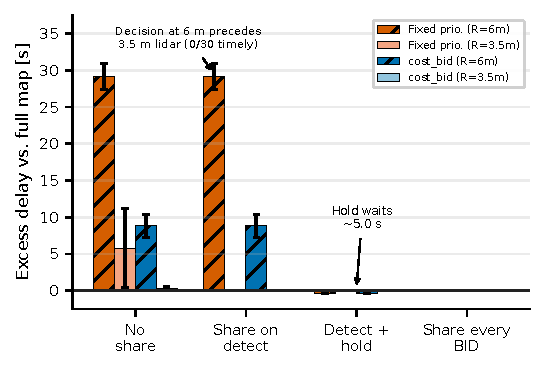
\includegraphics[width=\columnwidth]{Images/fig12_map_discovery.pdf}
\caption{Two-bay excess delay relative to full map knowledge in 2D \texttt{explore} mode ($0\%$ loss), showing why \texttt{share\_on\_detect} fails when radio negotiation ($R_{\mathrm{det}}=6$\,m) precedes $3.5$\,m Lidar range. Error bars show 95\% CIs.}
\label{fig:rq3_maps}
\end{figure}

\subsection{Three-Robot Topologies and Sim-to-3D Gazebo Transfer (RQ4)}\label{sec:rq4}
Pairwise negotiation rules must also handle multi-robot encounters where a third robot can physically block a yielding robot. In the 2-vs.-1 convoy study (1,080 episodes where follower~$C$ trails leader~$A$ against oncoming Robot~$B$, with 72 runs per policy and $B$-configuration pooled across $0\%$ and $50\%$ packet loss, Fig.~\ref{fig:rq4_convoy}), standard pairwise yielding traps a reversing leader against its own follower. Adding the local \texttt{make\_room} rule, which directs a blocking follower to back into an upstream refuge, eliminates all convoy deadlocks and achieves $72/72$ completion across every policy. The default rulebook, however, performs worst among the negotiating policies in every convoy regime ($40.0$\,s with equal robots, $100.1$\,s with loaded~$B$, and $133.6$\,s weighted with urgent~$B$, versus $33.7$, $33.7$, and $90.3$\,s for \texttt{fixed\_priority}), because its payload and urgency rules always make the two-robot convoy yield to a loaded or urgent lone robot, even when reversing the whole convoy is the costlier choice. When all robots have equal urgency ($u_A=u_C=u_B=1$), pairwise \cb\ only estimates the delay for leader~$A$ to reverse and ignores follower~$C$, resulting in an average delay of $55.6$\,s. Accounting for the whole convoy via \gb~\eqref{eq:groupbid} cuts mean delay to $34.4$\,s, coming within $+0.7\pm 1.4$\,s (paired difference) of both \texttt{fixed\_priority} and the hindsight side-level reference \texttt{side\_oracle} ($33.7$\,s). When the lone oncoming Robot~$B$ is urgent ($u_B=3$), however, \gb\ ($104.7\pm 6.7$\,s weighted delay) beats pairwise \cb\ ($117.1\pm 6.3$\,s, a paired improvement of $12.4\pm 5.8$\,s) but falls behind \texttt{fixed\_priority} ($90.3\pm 4.2$\,s, a paired gap of $+14.4\pm 8.0$\,s) and \texttt{side\_oracle} ($85.7\pm 3.1$\,s, a paired gap of $+19.0\pm 6.9$\,s). Because Eq.~\eqref{eq:groupbid} simply adds the individual yield delays of $A$ and $C$ together instead of modeling the extra time leader~$A$ must wait while follower~$C$ reverses out of the way first, \gb\ underestimates how long the convoy takes to yield and occasionally makes the convoy yield when backing lone Robot~$B$ into a nearby bay would actually be faster.

\begin{figure}[!t]\centering
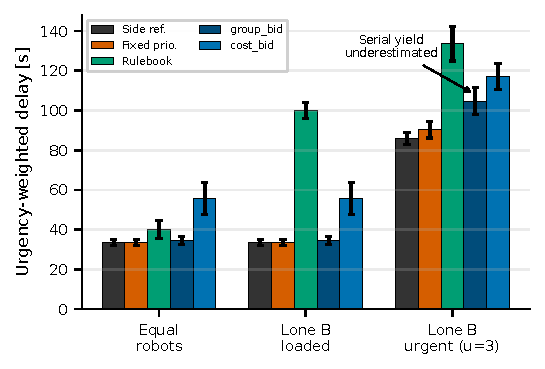
\includegraphics[width=\columnwidth]{Images/fig13_convoy_delay.pdf}
\caption{Convoy 2-vs.-1 urgency-weighted delay ($N=1{,}080$) across equal, loaded-$B$, and urgent-$B$ ($u_B=3$) regimes with follower \texttt{make\_room}. Error bars show 95\% CIs.}
\label{fig:rq4_convoy}
\end{figure}

\begin{figure}[!t]\centering
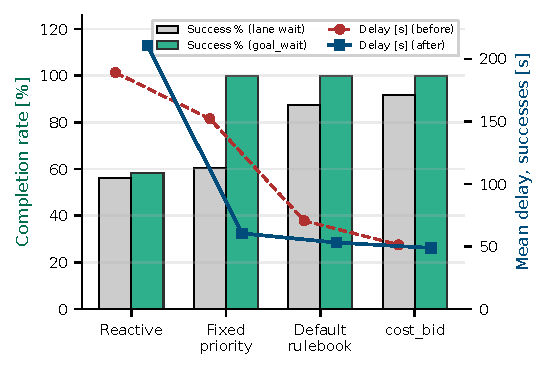
\includegraphics[width=\columnwidth]{Images/fig14_tjunction_goalwait.pdf}
\caption{Three-robot T-junction turn-in completion rate (bars, left axis) and successful-episode delay (lines, right axis) at $0\%$ loss ($n=48$ per policy) before versus after adding upstream bay waiting (\texttt{goal\_wait}).}
\label{fig:rq4_tjunction}
\end{figure}

A similar three-robot bottleneck occurs at branch intersections. In the T-junction turn-in study (384 episodes where Robot~$A$ is heading into branch \texttt{bay1} while Robot~$S$ is still inside \texttt{bay1} and Robot~$B$ is driving down the main corridor, with 48 runs per policy and packet-loss level, Fig.~\ref{fig:rq4_tjunction}), letting Robot~$A$ wait in the main corridor while \texttt{bay1} was occupied caused \texttt{fixed\_priority} to deadlock in $19/48$ runs ($60.4\%$ completion) at $0\%$ packet loss. Adding the \texttt{goal\_wait} rule, which directs Robot~$A$ to pull into the upstream refuge \texttt{bay0} until its target branch \texttt{bay1} clears, raised completion to $48/48$ ($100\%$) at both $0\%$ and $50\%$ packet loss for \texttt{fixed\_priority}, \texttt{rules\_default}, and \cb\ (compared with only $28/48$ for \texttt{reactive}, where all failures were deadlocks). With \texttt{goal\_wait} enabled at $0\%$ packet loss, mean total delay dropped from $60.5\pm 4.7$\,s under \texttt{fixed\_priority} to $53.1\pm 5.0$\,s under \texttt{rules\_default} and $48.9\pm 4.0$\,s under \cb\ (a paired improvement of $-4.3\pm 2.8$\,s over the rulebook).

Finally, to test whether the 2D results hold up under 3D rigid-body physics, planar LaserScan wall-filtering, and asynchronous ROS~2 message timing\label{sec:gz}, transfer was evaluated across 460 main validation runs in Gazebo Harmonic covering every study above (6 to 10 seeds per condition, taking $\sim 5$\,min of wall-clock time per episode including launch and reset) plus an additional 36-run explore-hold batch. Every Gazebo run was paired with a 2D simulation run using the exact same random seed (Table~\ref{tab:gz} and Fig.~\ref{fig:rq4_gz_scatter}). Within the 460-run main batch, 122 runs were executed on the code commit right before the explore and blocked-bay world features were added, and 338 were executed on the final commit (which did not change any behavior on default configurations), while all 36 hold-batch runs were executed on the final merged commit.

\begin{table}[!t]\centering
\caption{Seed-paired ROS~2 Jazzy / Gazebo Harmonic transfer summary (460 main validation runs + 36 hold/rerun batch runs).}
\label{tab:gz}
{\footnotesize\setlength{\tabcolsep}{3.0pt}
\begin{tabular}{@{}lrrrrr@{}}\toprule
Scenario / Study Group & Runs & Succ. & Coll. & Same & $\Delta D$ [s] \\\midrule
Single bay, negotiating (\texttt{S1}, S, L) & 70 & 70 & 0 & 70 & $-0.4$ \\
Single bay, \texttt{reactive}               & 10 &  9 & 1 &  5 & $-1.5$ \\
Forced yielders, S1 + S2 (O)             & 44 & 44 & 0 & 44 & $-0.5$ \\
Asymmetric urgency / speed (\texttt{S2}, neg.)    & 36 & 36 & 0 & 36 & $-0.6$ \\
Two bays (\texttt{S4})                      & 30 & 30 & 0 & 30 & $-0.2$ \\
Noisy bids ($\sigma=0.5, 1.0$; \texttt{S7}) & 12 & 12 & 0 &  7 & $+2.2$ \\
Clarke VCG misreports (\texttt{S9})         & 18 & 18 & 0 & 18 & $-0.3$ \\
50\% loss, $0.5$\,s latency (\texttt{S3})   & 18 & 18 & 0 & 18 & $-0.8$ \\
90\% loss, $2.0$\,s latency (\texttt{S8b/c})& 24 & 24 & 0 & 18 & $+4.8$ \\
Convoy 2 vs.\ 1 (\texttt{make\_room})       & 36 & 36 & 0 & 36 & $-0.6$ \\
T-junction (18 exit + 18 turn-in)           & 36 & 36 & 0 & 35 & $-16.8$ \\
Asymmetric static maps                      & 24 & 24 & 0 & 24 & $-0.3$ \\
Physically blocked bay                      & 18 & 18 & 0 & 18 & $-1.2$ \\
Explore (base, $R_{\mathrm{det}}\in\{6,3.5\}$) & 84 & 84 & 0 & 83 & $+0.2$ \\\midrule
\emph{Batch 2:} \texttt{hold\_for\_map}     & 24 & 24 & 0 & 24 & $+10.0$ \\
\emph{Batch 2:} \texttt{det\_3.5} rerun     & 12 & 12 & 0 & 11 & $+3.4$ \\\bottomrule
\end{tabular}}\\[2pt]
{\footnotesize Same: identical first yielder to paired 2D run (fixed by construction on forced runs). $\Delta D$: mean Gazebo minus 2D urgency-weighted delay over paired successes.}
\end{table}

Across all $450$ non-reactive main runs and all $36$ hold-batch runs ($486$ runs total), Gazebo recorded \emph{zero deadlocks and zero collisions} ($95\%$ upper bound of $0.85\%$ across the 450 main runs), whereas the non-communicating \texttt{reactive} baseline suffered 1 collision in 10 Gazebo runs. Leaving aside the 44 forced-yielder reference runs, $394$ out of $406$ negotiating runs ($97.0\%$, Wilson 95\% CI [94.9, 98.3]\%) picked the exact same first yielder in Gazebo as in their paired 2D run. Eleven of the 12 disagreements came from random noise that differed between the two simulators, namely, 5 noisy-bid runs (where the random bid noise is seeded using the rounded decision timestamp \texttt{round(t,1)}, which shifts slightly under asynchronous ROS~2 timing) and 6 runs at $90\%$ packet loss (which included tests with all safeguards on versus all off at $0.26$\,m/s). The 366 straight-corridor runs that shared identical random draws (blue circles in Fig.~\ref{fig:rq4_gz_scatter}) cluster tightly along $y=x$, and in the 116 single-bay and \texttt{S2} runs that have their own Gazebo forced-yielder reference, Gazebo excess delay matched the 2D excess delay within $1.0$\,s for every policy (\texttt{fixed\_priority} $7.5$\,s vs.\ $7.6$\,s; \texttt{reservation} $15.2$\,s vs.\ $15.2$\,s; \texttt{learned} $5.1$\,s vs.\ $5.3$\,s; and both \cb\ and \texttt{clarke} at $0.0$\,s in both simulators).

\begin{figure}[!t]\centering
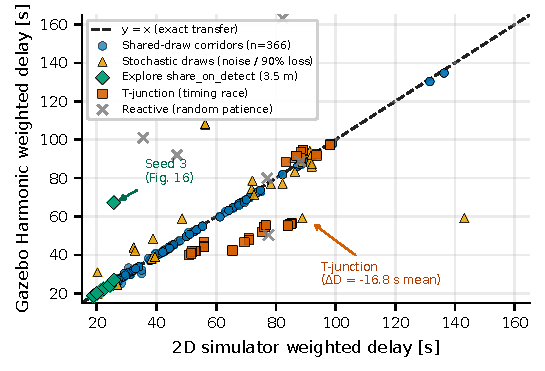
\includegraphics[width=\columnwidth]{Images/fig15_gazebo_scatter.pdf}
\caption{Paired Gazebo Harmonic versus 2D urgency-weighted delay across the 460-run main grid, showing tight clustering along $y=x$ for all 366 shared-draw corridor runs alongside isolated sim-to-3D divergence in T-junction timing races and $3.5$\,m \texttt{share\_on\_detect}.}
\label{fig:rq4_gz_scatter}
\end{figure}

Crucially, however, 3D Gazebo simulation revealed three physical and perceptual limits invisible in the 2D simulator.
\begin{enumerate}
\item \emph{Lidar peer-detection lag (\texttt{explore} and \texttt{hold\_for\_map}).} Whereas \texttt{sim2d} detects an oncoming robot immediately at $3.4$\,m inside the $3.5$\,m Lidar radius, Gazebo's wall-filtered \texttt{LaserScan} clustering ($0.35$\,m cluster distance matched within $2R_{\mathrm{sw}}=0.50$\,m of peer \texttt{STATE}) only registers an oncoming Waffle at $2.3$--$2.6$\,m separation on average. Consequently, even at $R_{\mathrm{det}}=3.5$\,m, \texttt{share\_on\_detect} delivered $0/6$ maps before decision time in Gazebo versus $6/6$ in 2D (Fig.~\ref{fig:rq4_gz_trace}), adding $+7.0$\,s of mean delay to \texttt{fixed\_priority} over the full-map Gazebo baseline ($+6.8$\,s over 2D). This mean is driven by a single run: on Seed~3, Robot~$B$ was sent to \texttt{room\_hi} ($+41.7$\,s), whereas in the other five runs the robots still chose \texttt{bay1} and Gazebo delay stayed within $0.2$\,s of the full-map baseline. Enabling \texttt{hold\_for\_map} (24 Gazebo runs) recovered the closer refuge (\texttt{bay1}) in $24/24$ runs, but peer detection occurred even closer ($1.10$--$1.18$\,m, waiting $4.7$\,s at $3.5$\,m and $9.5$\,s at $6.0$\,m), adding $+10.0$--$10.1$\,s over the full-map baseline. By then, Robot~$A$ ($6/6$) and Robot~$B$ ($5/6$) had already driven close enough to sense both bays directly, so holding worked in 3D by delaying the decision rather than by sharing maps. Including known bays in every \texttt{BID} (\texttt{share\_map}) avoids this lag entirely.
\item \emph{Branch-wall Lidar occlusion.} Early Gazebo T-junction runs showed that the $2.0$\,m side-branch walls block a parked branch robot's Lidar view of the main aisle (and exposed missing wall checks on room goals in 2D). Fusing fresh \texttt{STATE} positions into lane-clearance checks resolved this issue, meaning the final T-junction Gazebo runs serve as a post-fix verification rather than a blind transfer test.
\item \emph{Three-robot T-junction timing sensitivity ($\Delta D=-16.8$\,s).} Across all 36 T-junction runs, Gazebo accumulated $605.3$\,s less total delay than 2D ($-260.0$\,s across 18 exit runs and $-345.4$\,s across 18 turn-in runs). Event logs trace the exit gap (\cb\ $-264.7$\,s, \texttt{fixed\_priority} $+18.6$\,s, rulebook $-14.0$\,s) to a $\sim 20$\,s release-timing race. Under \cb\ in Gazebo, branch Robot~$S$ exits \texttt{bay1} slightly earlier while Robot~$A$ is still parked and slips past without triggering the second head-on conflict (or occasional $60$\,s proceed-timeout stall) seen in 2D, whereas under \texttt{fixed\_priority} and the rulebook, $S$ meets $A$ waiting in-lane and yields a second time ($4/4$ and $3/4$ runs). The larger turn-in offset ($9.5$--$28.9$\,s less delay per run and $0.4$--$6.4$\,s shorter makespan) remains an unexplained sim-to-3D timing gap, so exact T-junction delays cannot be predicted from 2D simulation alone.
\end{enumerate}

\begin{figure}[!t]\centering
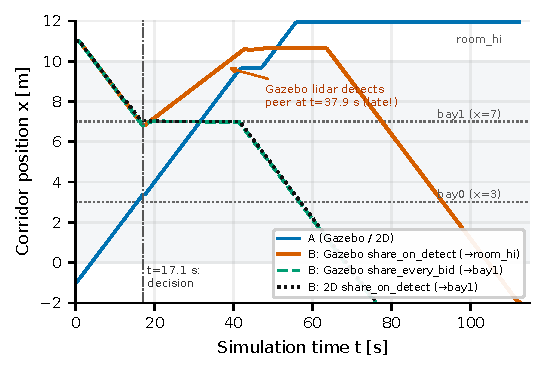
\includegraphics[width=\columnwidth]{Images/fig16_lidar_lag_trace.pdf}
\caption{Empirical spacetime trajectory $x(t)$ on Seed~3 ($R_{\mathrm{det}}=3.5$\,m): wall-filtered Gazebo Lidar clustering lags until $t=37.9$\,s, missing the $t=17.1$\,s decision window and sending $B$ to \texttt{room\_hi} instead of \texttt{bay1}.}
\label{fig:rq4_gz_trace}
\end{figure}